\documentclass{article}
\usepackage[utf8]{inputenc}
\usepackage{amsmath}
\usepackage{graphicx}
\usepackage{hyperref}
\usepackage{listings}
\usepackage{xcolor}
\usepackage{geometry}
\usepackage{cite}
\usepackage{float}
\geometry{a4paper, margin=1in}
\title{A Machine Learning Approach to Fetal Health Prediction Using Cardiotocography Data}
\author{Du Xuanlin, Tian Yuchen, Wang Guanyu}
\date{\today}

\begin{document}
\maketitle
\begin{abstract}
This report presents a machine learning approach to identify fetal distress using cardiotocography (CTG) data. We explore various machine learning models and data engineering techniques to improve prediction accuracy. The  result demonstrates the effectiveness of the proposed approach in classsifying fetah health status into three categories: Normal, Suspect and Pathological.
\end{abstract}

\section{Introduction}

The cardiotocography (CTG) is a widely used apparatus for monitoring the fetal health status during pregnancy, due to its cost effectiveness and being not invasive \cite{huang2021investigating}. However, the interpretation of CTG data is often too subtle for clinicians to make accurate and timely decisions. Machines are able to read and analyse large amounts of data quickly and consistently. Due to this nature, we propose a machine learning model to assist human clinicians in identifying fetal distress.

\section{Model Design}
After evaluating several machine learning algorithms, including Random Forest (RF) and eXtreme Gradient Boosting (XGBoost), we employed the XGBoost classifier due to its superior performance in terms of accuracy and robustness. 
\section{Data Processing}
The dataset was obtained from the UC Irvine Machine Learning Repository \cite{cardiotocography_193}, which consists of 2126 samples with 22 features. The target variable is the tri-state fetal health status. The raw data set comes with some missing values, irrelavant feature, metrics, and imbalanced class distribution. We performed data cleaning, feature selection and techniques such as SMOTE to address these issues.

The data process pipeline includes:

\begin{itemize}
	% BEST_COMBINAION = ['LB', 'AC', 'FM', 'UC', 'DS', 'DP', 'ASTV', 'MSTV', 'ALTV', 'Nzeros']
	\item Data Cleaning: Removing rows with missing values.
	\item Feature Selection: Out of the 22 feature, we preserved 10 features that are most relevant to fetal health status. We tried all possible combinations of these features and selected the best one based on cross-validation results. They are: \texttt{LB, AC, FM, UC, DS, DP, ASTV, MSTV, ALTV, Nzeros}.
	\item Metrics Scaling: We employed StandardScaler to unify the metrics scale of features.
	\item Handling Imbalanced Data: We applied SMOTE (Synthetic Minority Over-sampling Technique) to balanced the under-represented classes, Suspect and Pathological.
\end{itemize}

\section{Clinical Reasoning}

The following figure illustrates the importance of each feature in the model.

\begin{figure}[H]
	\centering
	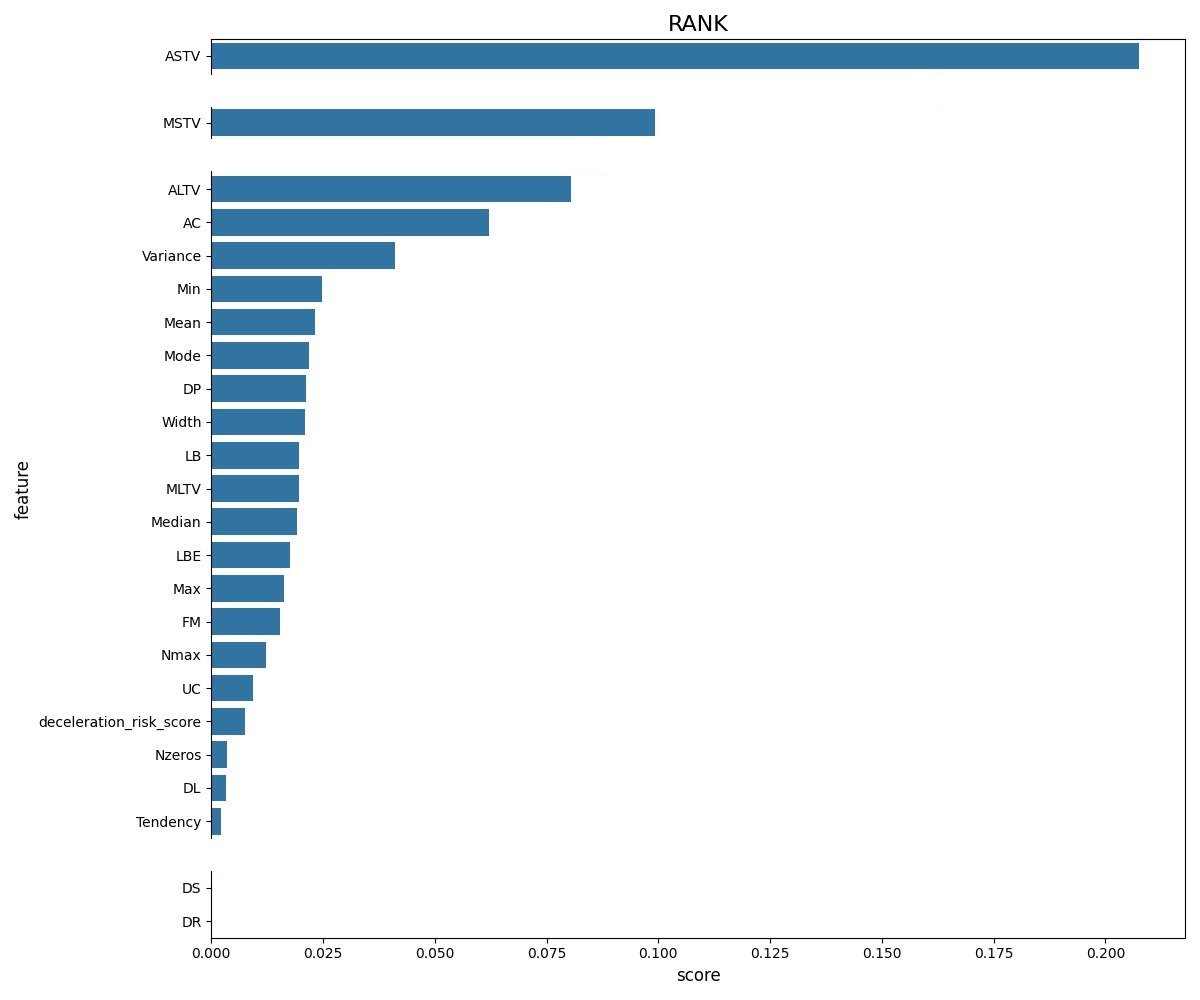
\includegraphics[width=0.8\textwidth]{dis.jpeg}
	\caption{Feature Importance}
\end{figure}

It can be seen that they coincide with the experiment result quite well, which means that the 10 features we selected are indeed nearly the most relevant ones to fetal health status, where the most significant driving features is \texttt{ASTV} (Percentage of Time with Abnormal Short Term Variability). Clinically, \texttt{ASTV} is a crucial indicator of fetal health status. As it increases, it often signifies a higher risk of pathological conditions \cite{huang2021investigating}. Therefore, it could be crucial for clinicians to monitor the \texttt{ASTV} feature closely when assessing fetal health status.

\section{Experiment Result}

After trainging and evaluating the effectiveness of the model using 5-fold cross-validation, we achieved on average a balanced accuracy of $0.891$ and a macro F1 score of $0.893$. 

\section{Conclusion}

This report presents a machine learning approach to identify fetal distress using cardiotocography data. By employing the XGBoost classifier and maintaining a good data hygiene, we achieved a good performance in terms of accuracy and robustness. The model can assist clinicians in making timely and relatively accurate decisions regarding fetal health status and providing a clinically interpretable reasoning. However, further polishing and validation on larger datasets and real-world testings are necessary before deploying the model in clinical settings. Human oversight is still required to ensure the medical safety.

\bibliographystyle{plain}
\bibliography{references}
\end{document}